\documentclass[a4paper,12pt, catalan]{book}

\usepackage[utf8]{inputenc}
\usepackage{babel}
\usepackage[backend=biber]{biblatex}
\bibliography{bibliografia/previ.bib}
\usepackage[dvips]{graphicx}
\usepackage{setspace}
\usepackage{times}
\usepackage{pdfpages}
% Fa que el ToC i els cites crein un link a on estan definits.
\usepackage{hyperref}
\usepackage{verbatim}
%\usepackage{pgfgantt}
%\usepackage{geometry}
%\geometry{verbose,a4paper,tmargin=25mm,bmargin=25mm,lmargin=3cm,rmargin=2cm}
\usepackage{titlesec} % Para modificar la apariencia de los titulos
\newcommand{\bigrule}{\titlerule[0.5mm]}
\titleformat{\chapter}[display] % cambiamos el formato de los capítulos
{\bfseries\Huge} % por defecto se usarán caracteres de tamaño \Huge en negrita
{% contenido de la etiqueta
 \titlerule % línea horizontal
 \filleft % texto alineado a la derecha
 \Large\chaptertitlename\ % "Capítulo" o "Apéndice" en tamaño \Large en lugar de \Huge
 \Large\thechapter} % número de capítulo en tamaño \Large
{0mm} % espacio mínimo entre etiqueta y cuerpo
{\filleft} % texto del cuerpo alineado a la derecha
[\vspace{0.5mm} \bigrule] % después del cuerpo, dejar espacio vertical y trazar línea horizontal gruesa

\spacing{1.3}
\AtBeginDocument{\let~=\nobreakspace}
\makeatother
\begin{document}
\pagestyle{empty}
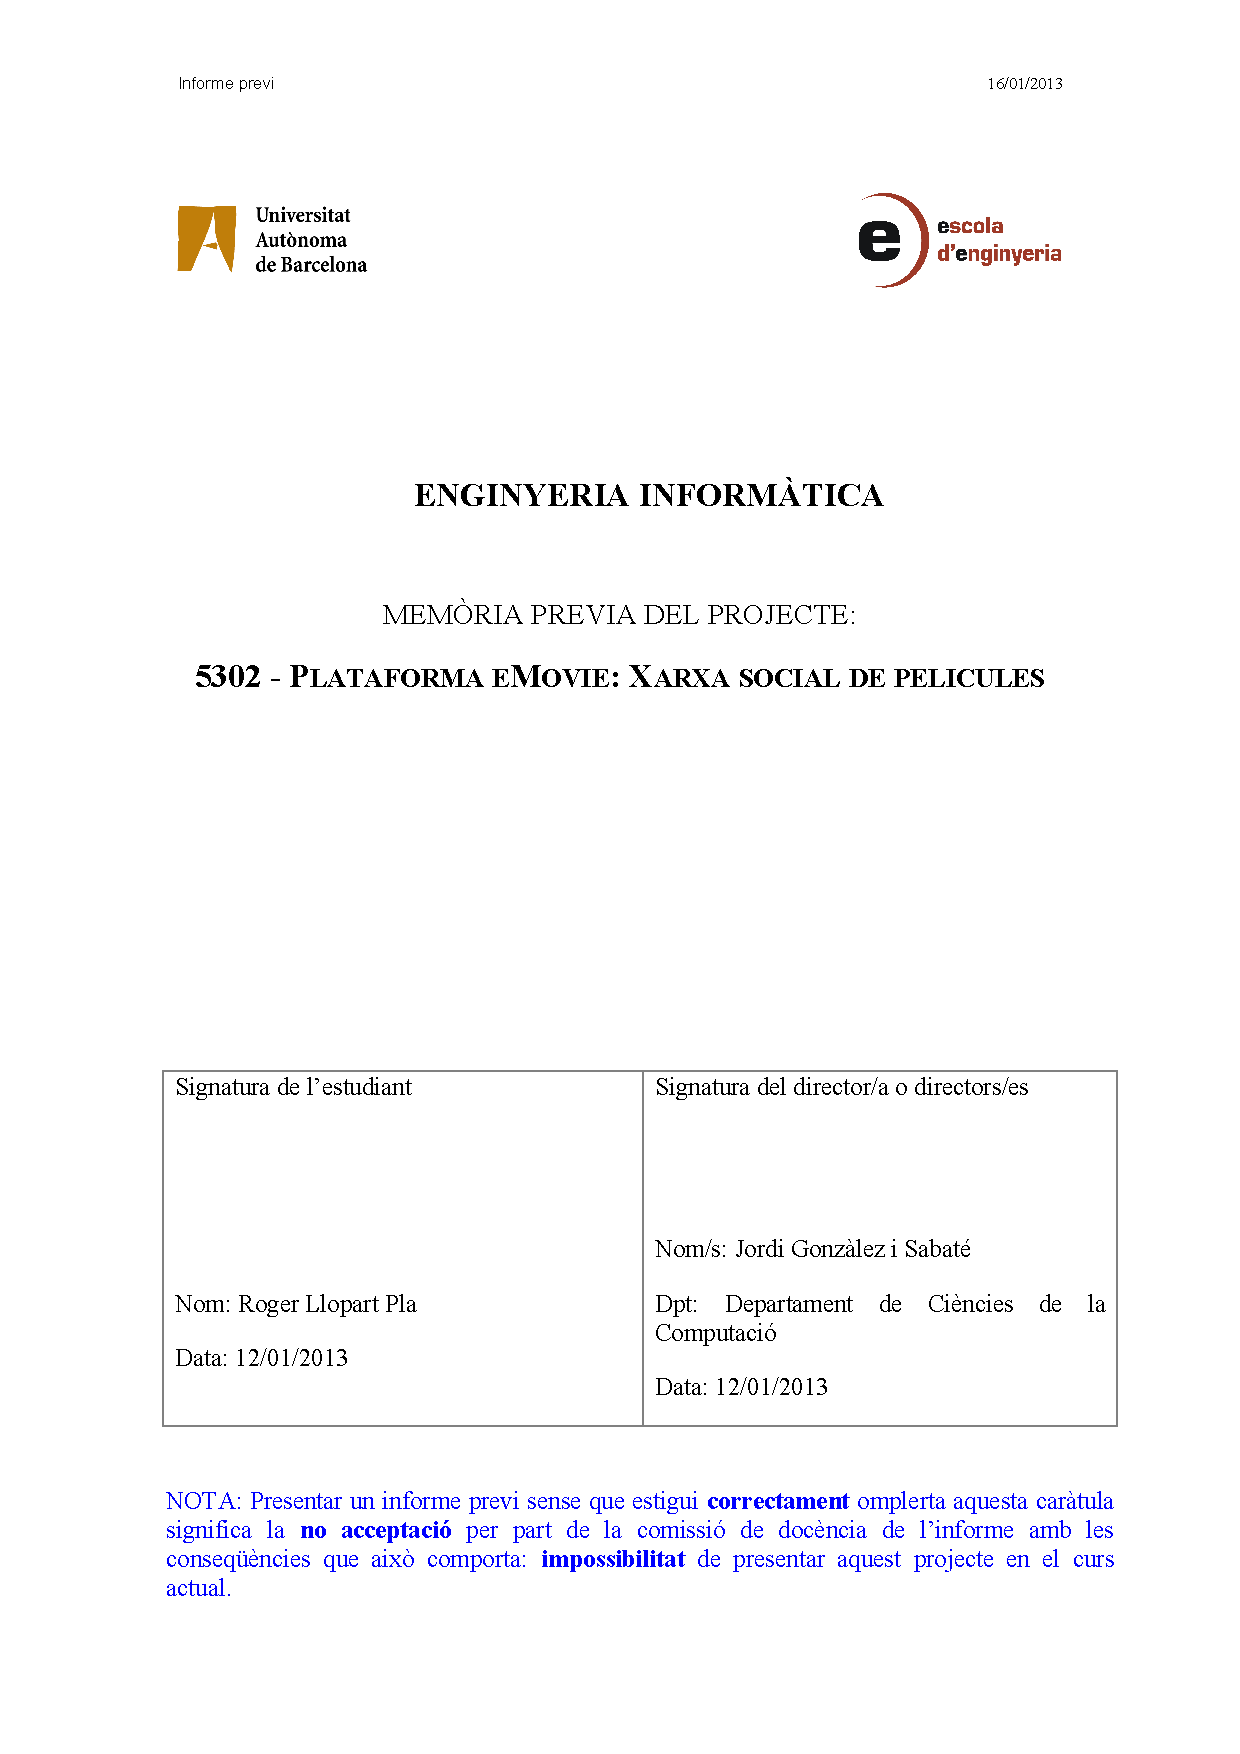
\includepdf{pdf/Portada.pdf}
\cleardoublepage
\pagestyle{plain}
\pagenumbering{roman}
\tableofcontents
\cleardoublepage
\pagenumbering{arabic}
\pagestyle{headings}
\chapter{Objectius}

L'objectiu d'aquest projecte seria la creacció d'una xarxa social amb temàtica orientada als llibres. El primer objectiu d'aquest aplicatiu web, el qual es busca dur a terme durant el desenvolupament d'aquest Projecte de Final de Carrera, seria, doncs implementar aquest recomanador. Per a implementar-lo, l'objectiu sería fer-ho amb una {\bf xarxa neural}.

Aleshores, es podria separar l'objectiu d'aquest projecte, en dues parts:

\begin{itemize}
\item Desenvolupament de l'interficie web: S'haurà de desenvolupar tota una interficie web amb la que l'usuari pugui interactuar. Aquesta requerirà d'unes parts que seràn explicades més en detall en un capitol de la memòria final, que serien un ACL\footnote{\textit{Access Control List}: Llista de Control d'Access}, un sistema per a la inserció de llibres i un altre sistema per a mostrar la informació sobre el llibre i es pugui marcar com a llegit.
\item Sistema recomanador: El sistema recomanador, que en principi serà una Xarxa Neural. S'haurà de fer un analisis sobre quines dades donar a la xarxa neural per tal de poder donar bones recomanacions.
\end{itemize}

No és segur que es pugui implementar un bon recomanador per mitjà d'una xarxa neural, per tant l'objectiu del projecte es podria considerar, també, el demostrar la viabilitat de l'ús d'una xarxa neural com a sistema per a implementar un recomanador de llibres.
\chapter{Estat de l'art}

\section{Algorismes de recomanació}

Els algorismes de recomanació són algorismes, que, com el seu nom indica, són emprats per a recomanar algúna cosa a algún individu. Aquesta definició, per simple que pugui semblar, introdueix dos elements molt importants. Introdueix el concepte de l'element a ser recomanat, d'ara en endavant el \emph{producte}, i el concepte de qui rep la recomanació, d'ara en endevant, l'\emph{usuari}. Des d'aquest punt, apareixeràn aleshores tres mètodes per atacar el problema d'aconseguir una recomanació de qualitat:

\begin{itemize}
	\item Recomanadors col·laboratius \\
		Aquests recomanadors es basen en tenir un conjunt d'\emph{usuaris} que valorin els \emph{productes} i, amb aquesta informació, determinen usuaris similars entre ells. Aleshores recomenarà a l'\emph{usuari} aquells \emph{productes} que hagin agradat als \emph{usuaris semblants} amb ell. El principal problema que tenen aquests recomanadors és que pateixen molt a l'inici del projecte, ja que cal tenir informació de molts \emph{usuaris} i molts \emph{productes} per tal de proveïr recomanacions encertades.
	\item Recomanadors basats en contingut \\
		Aquest altre sistema el que fa és categoritzar els \emph{productes}. Aleshores, quan l'usuari indica quins \emph{productes} li agraden, sap quines son les característiques més importants per a aquest \emph{usuari}.
	\item Recomanadors híbrids \\
		Aquest sistema consisteix en intentar unir els recomanadors col·laboratius amb els recomanadors basats en contingut. És el sistema més complex, donada la gran quantitat de variables que hi participen, però alhora també és el sistema que pot arribar a donar millors resultats, si es ben implementat i parametritzat.
\end{itemize}

\subsection{Recomanació de pel·lícules}

Existeixen moltes webs que es dediquen a la recomanació de pel·lícules. Per a acotar l'anàlisi de les tècniques que es fan servir reduirem el conjunt a 10.\cite{top-ten-film-recommenders}

Com havíem comentat a la secció anterior, es pot distingir fàcilment entre els \emph{recomanadors col·laboratius} i els \emph{recomanadors basats en contingut}. Exemples del primer conjunt podrien ser, per exemple, Netflix, Movielens, Flixter i Criticker. Per altra banda, formarien part del segon conjunt webs tals com Rotten Tomatoes i Jinni. Finalment, hi ha un tercer conjunt que són els que es basen en rebre com a input una pel·lícula i retornar-ne d'altres. Aquestes webs, com serien IMDb, Clerkdogs o Nanocrowd, molt probablement es basen en un \emph{recomanador basat en contingut} el qual extreu les característiques de la pel·lícula mencionada i en busquen d'altres que tinguin paràmetres similars.

\section{Importància de la recomanació a la web}

La recomanació a la web, que fins fa un temps no era massa comuna, cada cop està guanyant més importància tot i que no en siguem conscients. Un dels grans exemples de recomanació a internet és la publicitat. Un altre gran exemple de recomanacions el trobem als e-commerce, on fins i tot ja hi ha empreses de tercers que es dediquen a implementar els sistemes de recomanació, evitant així al desenvolupador del comerç on-line aquesta feina \cite{brainsins}.

Un exemple que és interessant de remarcar és \emph{Netflix}. Aquesta empresa va veure clar que els sistemes de recomanació eren importants, fins al punt que va organitzar un concurs on, els desenvolupadors que aconseguissin trobar el millor algorisme de recomanació, s'emportarien un premi d'un milió de dòlars \cite{netflix-prize}.

\section{Conjunt de proves}

Per a poder provar els diferents recomanadors que s'utilitzaran cal un conjunt de proves. Donat que, encara que es publiquès la web, aconseguir un conjunt de proves suficientment gran és un procès lent, s'ha utilitzat un conjunt de proves bastant comú en el camp de la recomanació, el de Movielens \cite{movielens-dataset}.

Movielens ha posat a disposició pública tres conjunts de dades diferents, un de cent mil puntuacions, un de un milió de puntuacions, i un de deu milions. El de deu milions té la limitació de que no han donat informació sobre els usuaris mentres que els altres dos conjunts si que en contenen.
\chapter{Viabilitat del projecte}

En aquesta secció es demostrarà com, a priori, aquest projecte és viable com a projecte de final de carrera.

\section{Viabilitat tècnica}

El desenvolupament d'aquesta aplicació en un entorn web implica una limitació molt important, que és el requisit de una resposta ràpida. Tot i així, com ja hem comentat a la secció~\ref{sec:estat-de-lart-ann}, aquest requisit es possible de complir-lo.

Apart d'aquest impediment de caràcter técnic, com el camp de l'aprenentatge màquina es un camp que ha estat bastant estudiat, no hauria de representar gaire problema el trobar implementacions ja fetes dels algoritmes que siguin necessaris per a dur a terme aquest sistema. I en cas de no trobar-lo desenvolupat, els algoritmes d'aprenentatge màquina són coneguts. Per tant, doncs, la dificultat d'aquesta aplicació serà en trobar els paràmetres correctes per al sistema, i no en l'implementació.

\section{Viabilitat econòmica}

Donat que tota aplicació que sigui utilitzada durant el projecte tindrà llicencia OpenSource o, com a mínim, permetrà el seu ús de forma gratuita per a projectes d'aquest tipus, l'únic cost del desenvolupament d'aquest projecte seràn les hores dèdicades i el cost de l'impresió de memòries, costos impossibles d'evitar en qualsevol projecte de final de carrera.

\section{Viabilitat legal}

El projecte no té cap característica d'ambit legal que calgui destacar.

\section{Alternatives}

Tot i que els estudis mencionats a la secció~\ref{sec:estat-de-lart-ann} demostren que és viable el desenvolupament d'una aplicació de recomanació web basada en una xarxa neuronal, en cas de no aconseguir realitzar l'implementació, existeixen sistemes per a realitzar \emph{Filtratge Colaboratiu}\cite{collaborative-filtering} sense necesitat de xarxes neuronals. Un exemple d'eina de codi lliure d'aquest tipus seria Apache Mahout\cite{Apache-Mahout}.

\section{Conclusions}

El projecte no presenta impediments a nivell tècnic, econòmic ni legal, i té una base prou ferma com per a poder concluir que és un projecte viable.
\chapter{Planificació temporal}

INCOMPLET
\begin{comment}
\section{Anàlisi del problema}

La planificació temporal d'aquest primer periòde, com es pot veure a la taula \ref{llegenda-gantt-analisi}, es centra únicament en estudiar que es el que s'ha fet fins al moment, i per on sería millor tirar per a desenvolupar aquesta aplicació.

\begin{table}[h!]
	\caption{Llegenda del diagrama de Gantt \ref{gantt-analisi}}
	\label{llegenda-gantt-analisi}
	\begin{center}
		\begin{tabular}{| c | c |}
			\hline
			{\bf Identificador}	& {\bf Descripció} \\ \hline
			1					& Estudi de l'estat de l'art \\
			2					& Diseny de l'aplicació \\
			3					& Estudi de les tecnologies a utilitzar \\
			4					& Redacció de l'informe previ \\ \hline
		\end{tabular}
	\end{center}
\end{table}

\begin{figure}[h!]
	\caption{Gantt de l'anàlisi del problema}
	\label{gantt-analisi}
	\begin{center}
		\begin{ganttchart}[vgrid]{14}
			\gantttitle{2011}{12}
			\gantttitle{2012}{2} \\
			\gantttitlelist{41,...,52}{1}
			\gantttitlelist{1,...,2}{1} \\
			\ganttbar{1}{1}{4} \\
			\ganttlinkedbar{2}{5}{9} \\
			\ganttlinkedbar{3}{10}{12} \\
			\ganttlinkedbar{4}{13}{14}
		\end{ganttchart}
	\end{center}
\end{figure}

\clearpage
\section{Desenvolupamnet de l'aplicatiu web}

La planificació de temps d'aquest segon periòde es centra en el desenvolupament de l'aplicació. Ho he dividit en les parts més representatives d'aquesta. Si es donés el cas de falta de temps, la tercera tasca, insercció de llibres de forma automàtica, seria deixada pel final, ja que, tot i ser bastant necesària per poder probar be l'aplicació, no és vital per al desenvolupament d'aquesta.

\begin{table}[h!]
	\caption{Llegenda del diagrama de Gantt \ref{gantt-desenvolupament}}
	\label{llegenda-gantt-analisi}
	\begin{center}
		\begin{tabular}{| c | c |}
			\hline
			{\bf Identificador}	& {\bf Descripció} \\ \hline
			1					& Login \\
			2					& Insercció de llibres manual \\
			3					& Insercció de llibres automàtic \\
			4					& Buscador \\
			5					& Estudi sobre recomanadors \\
			6					& Implementació del recomanador \\ \hline
		\end{tabular}
	\end{center}
\end{table}

\begin{figure}[h!]
	\caption{Gantt del desenvolupament de l'aplicatiu web}
	\label{gantt-desenvolupament}
	\begin{center}
		\begin{ganttchart}[vgrid]{22}
			\gantttitle{2012}{22} \\
			\gantttitlelist{3,...,24}{1} \\
			
			\ganttbar{1}{1}{2} \\
			\ganttlinkedbar{2}{3}{4} \\
			\ganttlinkedbar{3}{5}{7} \\
			\ganttlinkedbar{4}{9}{11} \\
			\ganttlinkedbar{5}{12}{15} \\
			\ganttlinkedbar{6}{16}{22}
		\end{ganttchart}
	\end{center}
\end{figure}
\end{comment}
\chapter{Altres comentaris}

No hi ha més comentaris a fer.
\cleardoublepage
\phantomsection
\addcontentsline{toc}{chapter}{Bibliografia}
\printbibliography
\end{document}